\section{Zmienne}

\begin{frame}[fragile]
  \frametitle{Zmienne}
  \framesubtitle{Definicja}

  \textbf{Zmienna} (ang. variable) jest magazynem z nazwą dla danych.

  \begin{itemize}
    \item służą do przechowywania danych
    \item podobnie jak w języku \textbf{Python} ich typ jest dynamiczny
    \item deklaracja zmiennej przez słowo kluczowe \verb|let|
  \end{itemize}

  \begin{minted}{js}
    let imie;
    let wiek = 15;
  \end{minted}
\end{frame}


\begin{frame}[fragile]
  \frametitle{Zmienne}
  \framesubtitle{Definicja}

  Nazwa zmiennej ma pewne ograniczenia:

  \begin{itemize}
    \item moża zawierać tylko: litery, cyfry oraz znaki \$ \_
    \item pierwszym znakiem nie może być cyfra
  \end{itemize}
\end{frame}

\begin{frame}[fragile]
  \frametitle{Zmienne}
  \framesubtitle{Definicja}

  Prawidłowe nazwy zmiennych:
  \begin{minted}{js}
    let imie;
    let $nazwisko;
    let zmienna123;
    let login_lub_haslo;
    let nazwaUzytkownika;
  \end{minted}
\end{frame}


\begin{frame}[fragile]
  \frametitle{Zmienne}
  \framesubtitle{Definicja}

  Nieprawidłowe nazwy zmiennych:
  \begin{minted}{js}
    let 1imie;
    let imie nazwisko;
    let wiek%;
  \end{minted}
\end{frame}

\begin{frame}[fragile]
  \frametitle{Zmienne}
  \framesubtitle{Definicja}

  Nazwy zmiennych mogą posiadać polskie znaki:

  \begin{minted}{js}
    let imię;
    let czyObowiązkowy;
    let prędkość_maksymalna;
  \end{minted}

  \textbf{Ale uwaga! Dobrą praktyką jest unikanie używania polskich znaków.}
\end{frame}


\begin{frame}[fragile]
  \frametitle{Zmienne}
  \framesubtitle{Definicja}

  Deklaracja zmiennej odbywa się przy użyciu słowa kluczowego \verb|let|:

  \begin{minted}{js}
    let mojaZmienna;
  \end{minted}

  W trakcje deklaracji, zmienną możemy inicjalizować wartością przy użyciu operatora przypisania \verb|=|:

  \begin{minted}{js}
    let mojaZmienna = 'Ala ma kota';

    let mojaZmienna;
    mojaZmienna = 'Ala ma kota';
  \end{minted}
\end{frame}


\begin{frame}[fragile]
  \frametitle{Zmienne}
  \framesubtitle{Definicja}

  Ponowne przypisanie wartości do zmiennej, powoduje nadpisanie poprzedniej wartości:

  \begin{minted}{js}
    let mojaZmienna = 'Ala ma kota';  // Ala ma kota
    mojaZmienna = 'Ala ma psa';       // Ala ma psa
    mojaZmienna = 123;                // 123
  \end{minted}

\end{frame}


\begin{frame}[fragile]
  \frametitle{Zmienne}
  \framesubtitle{Definicja}

  Informacje powiązane ze zmiennymi, które w tej chwili pominiemy:

  \begin{itemize}
      \item słowo kluczowe \verb|var|
      \item zasięg zmiennych
  \end{itemize}
\end{frame}


\begin{frame}[fragile]
  \frametitle{Zmienne}
  \framesubtitle{Definicja}

  \verb|prompt(message, default)| --- wyświetla okno dialogowe do wprowadzania tekstu, zwraca wprowadzony tekst

  \begin{itemize}
      \item \verb|message| --- komunikat wyświetlany w oknie dialogowym 
      \item \verb|default| --- wartość domyślna pola 
  \end{itemize}
  
  \begin{minted}{js}
    let imie = prompt('Jak masz na imię?');
  \end{minted}

  \begin{figure}
    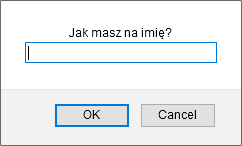
\includegraphics[scale=0.5]{images/js-prompt-example}
  \end{figure}
\end{frame}









